\documentclass[12pt,a4paper]{article}

% Useful packages for article:
\usepackage{amsmath, amssymb, amsfonts, amsthm}
\usepackage{graphicx}
\usepackage[round]{natbib}
\usepackage[usenames,dvipsnames]{xcolor}
\usepackage{bm}
\usepackage{subfigure}
\usepackage{graphicx}
\usepackage{mathabx}
\usepackage{multirow}
\usepackage{setspace}
\usepackage{tabls,calc}
\usepackage{float}
\usepackage{parskip}
\setcounter{tocdepth}{5}
\setcounter{secnumdepth}{5}
\numberwithin{equation}{section}
\numberwithin{figure}{section}
\numberwithin{table}{section}
\floatstyle{ruled}
\restylefloat{table}
\restylefloat{figure}

%Theorem, Lemma, etc. environments
\newtheorem{theorem}{Theorem}%[section]
\newtheorem{lemma}[theorem]{Lemma}
\newtheorem{proposition}[theorem]{Proposition}
\newtheorem{corollary}[theorem]{Corollary}
\newtheorem{result}[theorem]{Result}

\newcommand{\floatintro}[1]{

  \vspace*{0.1in}

  {\footnotesize

    #1

    }

  \vspace*{0.1in}
}
\usepackage[pdftex, pdfusetitle, plainpages=false, 
				letterpaper, bookmarks, bookmarksnumbered,
				colorlinks, linkcolor=Sepia, filecolor=Blue, urlcolor=Blue, citecolor=Violet]
				{hyperref}

\makeatletter

%%%%%%%%%%%%%%%%%%%%%%%%%%%%%%%%%%%%%%%%%%%%%%%%%%%%%%%%%%%%%%%%%%%%%%%
%
%  Floats
%
%%%%%%%%%%%%%%%%%%%%%%%%%%%%%%%%%%%%%%%%%%%%%%%%%%%%%%%%%%%%%%%%%%%%%%%%
%
%  \c@topnumber            : Number of floats allowed at the top of a column.
\setcounter{topnumber}{8}
%
%  \topfraction            : Fraction of column that can be devoted to floats.
\renewcommand\topfraction{1}
%
%  \c@bottomnumber, \bottomfraction : Same as above for bottom of page.
\setcounter{bottomnumber}{3}
\renewcommand\bottomfraction{.8}
%
%  \c@totalnumber          : Number of floats allowed in a single column,
%                          including in-text floats.
\setcounter{totalnumber}{8}
%
%  \textfraction         : Minimum fraction of column that must contain text.
\renewcommand\textfraction{0}
\renewcommand\floatpagefraction{.9}
%
%  \c@dbltopnumber, \dbltopfraction : Same as above, but for double-column
%                          floats.
\setcounter{dbltopnumber}{6}
\renewcommand\dbltopfraction{1}
\renewcommand\dblfloatpagefraction{.9}
%
\pretolerance=8000
\tolerance=9500
\hfuzz=0.5pt
\vfuzz=2pt
\hbadness=8000
\vbadness=8000
%\newcommand{\nohyphens}{\hyphenpenalty=10000\exhyphenpenalty=10000}
\def\endcolumn{\parfillskip=0pt\par\newpage
   \noindent\parfillskip=0pt plus 1fil{}}

\newsavebox\ruledbox
\newlength \ruledlength
\ruledlength\linewidth 
\newcounter{box}
\renewcommand \thebox{\@arabic\c@box}
\def\fps@box{tbp}
\def\ftype@box{1}
\def\ext@box{lob}
\def\boxname{Box}
\def\fnum@box{\boxname~\thebox}
\@ifundefined{color}{%
\newenvironment{thinbox}
 {\fboxsep6pt
  \setlength\ruledlength{\linewidth-2\fboxsep-2\fboxrule}
  \begin{lrbox}{\ruledbox}
   \begin{minipage}{\ruledlength}
   \def\@captype{box}}
 {\end{minipage}\end{lrbox}
  \@float{box}
   \fbox{\usebox{\ruledbox}}
  \end@float}
\def\endcolumn{\parfillskip=0pt\par\newpage
   \noindent\parfillskip=0pt plus 1fil{}}
% CVR's two-column box
\newenvironment{widebox}
 {\fboxsep6pt
  \setlength\ruledlength{\textwidth-2\fboxsep-2\fboxrule}
  \begin{lrbox}{\ruledbox}
   \begin{minipage}{\ruledlength}
   \def\@captype{box}}
 {\end{minipage}\end{lrbox}
  \@dblfloat{box}
   \fbox{\usebox{\ruledbox}}
  \end@dblfloat}
}{%
\definecolor{linecolor}{rgb}{0,0,.6}
\definecolor{bgcolor}{rgb}{1,.894,.769}
\newenvironment{thinbox}
 {\fboxsep6pt%\fboxrule2pt
  \setlength\ruledlength{\linewidth-2\fboxsep-2\fboxrule}
  \begin{lrbox}{\ruledbox}
   \begin{minipage}{\ruledlength}
   \def\@captype{box}}
 {\end{minipage}\end{lrbox}
  \@float{box}
   \fcolorbox{linecolor}{bgcolor}{\usebox{\ruledbox}}
  \end@float}
\def\endcolumn{\parfillskip=0pt\par\newpage
   \noindent\parfillskip=0pt plus 1fil{}}
% CVR's two-column box
\newenvironment{widebox}
 {\fboxsep6pt\fboxrule1pt
  \setlength\ruledlength{\textwidth-2\fboxsep-2\fboxrule}
  \begin{lrbox}{\ruledbox}
   \begin{minipage}{\ruledlength}
   \def\@captype{box}}
 {\end{minipage}\end{lrbox}
  \@dblfloat{box}
   \fcolorbox{linecolor}{bgcolor}{\usebox{\ruledbox}}
  \end@dblfloat}
}
\makeatother
  
\title{Deep Graph Kernels for Inferring Bitcoin Transactions Dynamics \thanks{Interim thesis report} }

\author{Pankaj Kumar\thanks{Skolkovo Institute of Science and Technology, Skolkovo Innovation Center, Building 3, Moscow  143026 Russia. Email: \url{pankaj.kumar@skolkovotech.ru}}} 


\date{}

\begin{document}
\maketitle
%\begin{abstract}
%
%\end{abstract}
%\par
%\noindent
%\textbf{Keywords:} Agent Based Model $\cdot$ High Frequency Trading $\cdot$ Agent Ecology $\cdot$ Trading Strategies $\cdot$ CDA \\
%\\
%\textbf{JEL Classification:} G10 $\cdot$ C12
%\newpage
%\tableofcontents
\newpage
\section{Introduction}
\label{sec:Introduction}
Bitcoin is a decentralized peer to peer electronic payment system in which transactions are performed with no central authority or banks to authorize it. The Bitcoin transactions management and its issuance is carried out collectively by the network. The first Bitcoin specification and proof of concept was published by Satoshi Nakamoto \citep{Nakamoto2009} in 2009 cryptographic mailing list. Since then, the community has grown exponentially with many developers working on Bitcoin.

Bitcoin payments use public keys encryption, where, payers and payees are identified by hashed public keys of their Bitcoin wallets. The public keys are generated by ECDSA (Elliptic Curve Digital Signature Algorithm), based on calculations of elliptical curves over finite space. Suppose, Alice sends "$x$" coins to Bob, then an unencrypted transaction attaching Bob's public key is broadcast over the Bitcoin network using her private key. The signature on transaction verifies all users for its authenticity (current owner of coin) by looking at complete history of transactions.



\subsection{Blockchain}
\label{subsec:Blockchain}

The complete record of transactions is in a coded form in a data structure called {\it blockchain}, which is a sequence of records called {\it blocks}. Each block contains a group of transactions that have been sent since the previous block, with integrity check all the way back to the first one, the genesis block.

Any users enter the Bitcoin system by trading non-digital currencies at Bitcoin market exchange, or by mining coins, which involves solving a cryptographically hard problem for which he/she is suitably rewarded a fixed number of Bitcoins  and transactions is validated on the network. The working of mining, core to {\it blockchain}, is mathematically explained better by \cite{Johannes2015}. 

At first, miner~$M$ computes a block hash~$h$ over a unique ordering
of the hashes of all the transactions that it is intending to incorporate into its next block $B$.  Then, input of the block solution $s_{i-1}$ is taken at the head of its current version of the {\it blockchain}. If we concatenate the strings by the symbol $+$, the cryptographic problem that $M$ has to solve is: compute a SHA-256 hash
%
\begin{equation} \label{eq:1.1}
s_i = (n + h + s_{i-1}),
\end{equation}
%
such that $s_i$ has at least a specified number~$x$ of leading zeros where $x \sim 64$. 

\subsection{Market \& Bitcoins}
\label{subsec:Market and Bitcoins}

Bitcoin started trading	 on Mt.	Gox, the largest online	 Bitcoin exchange at 5 cents. Over the next	 two	 years,	Bitcoin/USD exchange rose slowly, but in early April 2013, the price per bitcoin dropped from \$266 to around \$50 and then rose to around \$100. This major bubble was succeeded by another one on 29 Nov, 2013, when, the price of a bitcoin reached an all-time high of US\$1224.76 on 29 November 2013, then dropped into the \$200-\$300 range. Metaphorically, the price rise/drop is expressed as skippyball. Once skippyball pitched high in the air, the first bounce is big, then lower, and lower, until it is flat on the ground, ready for a new throw upward. Taking market price data from Blockchain the most popular Bitcoin wallet \footnote{Market Price in USD \url{https://blockchain.info/charts/market-price}}, the bubbles can be visualized in the time series plot \ref{fig:bubble} with circles representing bubbles.

\begin{figure}[ht]
\begin{center}
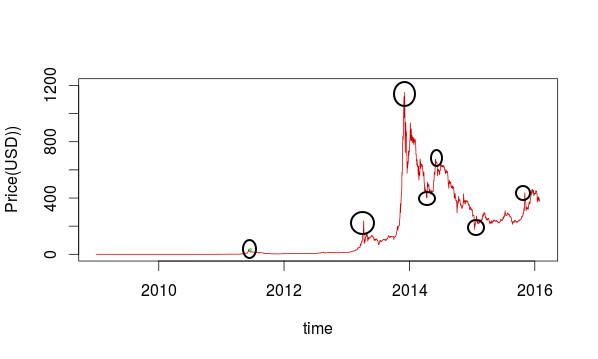
\includegraphics[width=\textwidth]{./figure/bubble.png}
\caption{Market Price (USD)}
\label{fig:bubble}
\end{center}
\end{figure} 

According to an economic explanation \citep{Lo2014, Kristoufek2015} for Bitcoin bubble in April, 2013, the financial crisis in Cyprus, triggered large numbers of people to converted their euros into digital Bitcoins. The real cause of the Bitcoin bubble and burst is still unexplored research territory , but it encourages researchers to model the the underlying system of interacting agents to gain a better understanding of the underlying phenomena. The first step in this direction would be to get transaction network, identify its structural parameters, like walk or path and find its correlation with market price. Then, comes the understating of the network behaviour to have concrete explanations to support any theory.

Using complete list of transactions, parsed from blockchain, \citet{Kondor2014} reconstructed transaction network and applied unsupervised identification to get the most important features of the time variation of the network. By applying Principal Component Analysis to the matrix constructed from
snapshots of the network at different times, they showed that structural changes in the network accompany significant changes in the exchange price of Bitcoins. The one fall-back about this paper is scalability, which makes it unsuitable for application having nodes greater than 10000 nodes \citep{Zager2008}.



\subsection{Graph Similarity \& Subgraph Matching}
\label{subsec: Graph Similarity}

The above solution proposed by \citet{Kondor2014} falls on the category of basic graph similarity and subgraph matching algorithms, which is not scalable with increasing number and the size of graphs (eg: bitcoin \ref{fig:transactions}). There are challenges on proposing meaningful metrics to capture different notions of structure, designing algorithms that can calculate these metrics, and finally finding approximations or heuristics to scale with graph size if the original algorithms are too slow.

\begin{figure}[ht]
\begin{center}
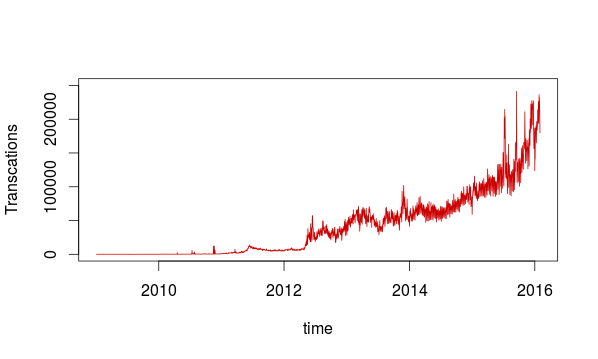
\includegraphics[width=\textwidth]{./figure/transactions.png}
\caption{Daily Transactions}
\label{fig:transactions}
\end{center}
\end{figure}

Most of graph isomorphism algorithms and its generalizations are exponential and, thus, not applicable to the large graphs that are of interest today. The other methods  for graph similarity and graph sub-matching, like features extractions, iterative methods and tensors analysis, including some come with their drawbacks \citep{Zager2008}.

In the recent paper on graph kernels, \citet{Yanardag2015} used "Deep Graph Kernels", a unified framework to learn latent representations of sub-structures for graphs to compare graphs. As Bitcoin transaction network graph is increasing everyday, It would be interesting to capture its structural dynamics by method proposed in the paper.


\subsection{Motivation}
\label{subsec:Motivation}

The volatile rise and fall of Bitcoin, cryptological mining, complex distributed database, blockchain and evolving network dynamics promoted me to  efficiently measures the structural change (eg. walks) of a dynamic large-scale graph as well as the similarity between two graphs with reference to price change. 

In simple words, the thesis attempts to address two important questions:  
\begin{enumerate}
\item How much is a daily bitcoin transaction graph transformed over time or by a significant event (bubbles)?
\item How structurally similar are two daily bitcoin transactions graphs ?
\end{enumerate}
 


\subsection{Objective}
\label{subsec:Objective}

The objective of thesis are following:
\begin{enumerate}
\item Given complex cryptic distributed blockchain, parsing it to extract transaction attributes in the form. \textcolor{red}{complete}

\begin{center}
\begin{tabular}{ |c|c|c|c| } 
 \hline
 $Transaction_{From}$ & $Transaction_{To}$ & $Value$ & $Timestamp$ \\ 
  \hline
\end{tabular}
\end{center}

\item Get daily transactions graphs. \textcolor{red}{complete}

\item Given two graphs $G_1 (n_1 , e_1 )$ and $G_2 (n_2 , e_2 )$, find an algorithm to calculate the similarity index between the two graphs. \textcolor{red}{partially complete}.

\item Given a graph time series, where there are $T$ number of graphs, find approximate subgraphs that occur in a subset of the $T$ graphs. \textcolor{red}{literature review complete}

\end{enumerate}



\section{Data}
\label{sec:data}

The blockchain is a transaction database of the Bitcoin.  Once Bitcoin core is setup at local machine, blockchain is automatically downloaded. Every full node participating in the Bitcoin network has the same copy. As of now there is more than 60 GB of Bitcoin blockchain dataset, which makes it difficult to parse the raw blockchain data. Most of the previous studies \citep{Ron2013} employed a forked version of bitcointools \footnote{\url{https://github.com/gavinandresen/bitcointools}}, but from the bitcoin clients 0.8 version, it indexed the full blockchain using LevelDB instead making the publicly available bitcointools obsolete. Other well know open source blockchain parser like blockparser \footnote{https://github.com/znort987/blockparser}, BitIodine \citep{Spagnuolo2013} etc are almost undocumented projects, where some appear to not even work. A paper \citep{Fleder2015} led me to BitcoinArmory project, which requires a dozen of manual interventions to get installed, but still doesn’t work.

We then started to look for ready-made SQL database, which pointed to BitcoinABe. This python based library reads the Bitcoin block file, transforms and loads the data into a SQL database. But, Its takes more than two weeks to dump the data, which was not feasible option. We downloaded postgres database dumps of the bitcoin-ruby-blockchain database generated by webbtc \footnote{\url{http://dumps.webbtc.com/bitcoin/}}. Then, with slight modification to open repository BitIodine \citep{Spagnuolo2013} code, we parsed through the blockchain, and wrote wrapper classes that extracted the relevant information required to construct the transaction graph. The market price data was scarped from website \url {https://blockchain.info/} to plot graphs in R.

\section{Bitcoin Transaction Netowrk}

With the overall transactions records parsed from the blockchain in human readable form, we construct a a weighted directed transaction graph that gives an intuition towards the flow of Bitcoins from one key to the other,the directed edge represents a particular transaction from a source address to a target address and weight represents the value of the transactions. For our experiments, we constructed graphs for 45 days between and after 10 April, which was first major bubble in Bitcoin history. we wanted to first confirm the correlation between market price and network dynamics, before proceeding to analyse whole data.

\begin{figure}[ht]
\begin{center}
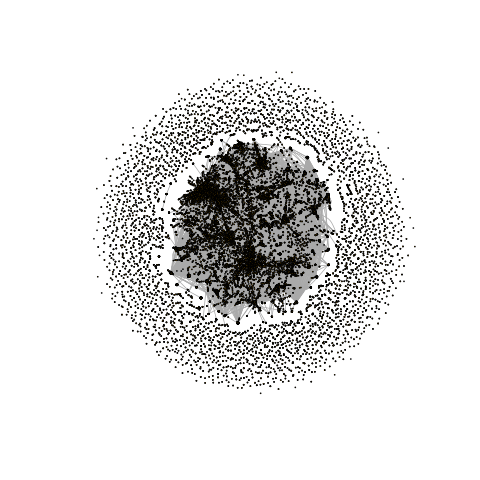
\includegraphics[width= 100mm]{./figure/dt.png}
\caption{ Daily transaction graph for a typical day (April 8, 2013)}
\label{fig:dt}
\end{center}
\end{figure}

\section{Graph Isomorphism}
Long in the purview of researchers, graph isomorphism is a well-studied problem in literature. There are several approaches proposed to solve variations of the problem. Though graph isomorphism is a classic open problem in the algorithmic theory of random graphs, but recent work by \citet{Babai2015} showed that it can be solved in in quasipolynomial ($\exp\left((\log n)^{O(1)}\right)$) time. Where, the best previous bound for graph isomorphism was $\exp(O(\sqrt{n\log n}))$;  $n$ is the number of vertices.

Another approach of attacking graph isomorphism is based on features extraction. The $\lambda$-distance, a spectral method and levenshtein distance which defines the distance between two graphs as the distance between their spectra (eigenvalues) has been studied thoroughly \citep{Koutra2013}. The study by \citet{Li2012} proposes an SVM-based approach on extracted features (average degree, eccentricity, number of nodes and edges, eigenvalues, clustering coefficient, diameter etc.) to perform graph isomorphism. Other techniques includes, computing edge curvatures under heat kernel embedding, comparing graph signatures consisting of
summarized local structural features  and a distance based on graphlet correlation \citep{Koutra2013}. Though these methods are powerful and scale well, but depending
on the statistics that are chosen, it is possible to get results that are not intuitive. For example, it is possible to get high similarity between two graphs with very different node set size, which is not always desirable. Adding to the same, feature vector transformation leads to loss of topological information.

Next approach is based on iterative methods, which is based on the concept to find the "best" correspondence between the nodes of the two graphs. The research direction attempting to solve the graph alignment problem is flooded with the methods span from genetic algorithms to decision trees, clustering, expectation-maximization, similarity flooding algorithm \citep{Melnik2002}, message-passing algorithm for aligning sparse networks and belief propagation \citep{Koutra2013}, to name few of them. The advantages of all enlisted methods are their speed and simplicity, but they do not take into account information about the graph structure. On graph similarly measure with given node correspondence, \citet{Koutra2013} proposed DELTACON , a principled, intuitive, and scalable algorithm that assesses the similarity between two graphs on the same nodes using Fast Belief Propagation on real graphs from ENRON e-mail exchange and brain scans. The specific application to node correspondence make its unsuitable for dynamic graphs.

Going in the research direction of tracking changes in networks over time, spotting anomalies and detecting events, \citet{Lee2015} graph similarity approach is based on random walk with restart (RWR) algorithm with intergraph compression to transform representation of graph. The method is efficient in space requirement and produces results more quickly and accurately over conventional graph transformation schemes. The methods fails in picking Euclidean distance as measurement of matrix distance, as it become weakly discriminant when we have multidimensional and sparse data. Another work by \citet{Mheich2015} on measure graph similarity takes account for vertices, edges and spatiality at the same time, which is unseen in literature.

Another important approach which work directly on the graphs without doing feature extraction is called graph kernels. It characterize graph features in a high dimensional space and thus better preserve graph structures. Most of graph kernels
are instances of the family of R-convolution kernels proposed by \citet{Haussler1999}, which define graph kernels by comparing all pairs of isomorphic substructures under decomposition, and a new decomposition
will result in a new graph kernel. It can be categorised into classes based on comparing all pairs of walks, paths, cycles \citep{Aziz2013}, trees and graphlets in polynomial time \citep{Vishwanathan2010}.

One of the popular graph kernel, random walk graph kernel \citep{Gartner2003, Kashima2003} counts matching walks in two input graphs. It is prohibitively expensive, requiring $O(n_{6})$ runtime and suffers from the problem of tottering and halting. The computation of the above was greatly improved by \citet{Vishwanathan2007} using iterative methods, including those based on Sylvester equations, conjugate gradients, and fixed-point iterations. Other improvements by \citet{Kang2012} takes account for just unlabeled graphs with the normalized weight matrix. Tottering problem was solved by \citet{Mahe2004} by doing special transformation on the input graphs, but it suffer from adverse computation time ($O(n)$ to $O(n_{2}$) and does not show a uniform improvement of classification accuracy. Replacing walk by path \citet{Borgwardt2005}, solved the tottering and  halting problem, but dense matrix representation for connected graphs, may lead to memory problems on large graphs. Adding to the same, the recent paper by \citet{Sugiyama2015} claimed geometric random walk kernels suffers from the problem  referred to as halting: Longer walks are downweighted so much that the similarity score is completely dominated by the comparison of walks of length 1.

Other graphs kernels too suffer from disadvantages. For example, Optimal Assignment Kernels and Edit-Distance Kernel are not positive definite in general; Subtree Kernel runtime grows exponentially with the recursion depth of the subtree like patterns; Cyclic Pattern Kernel restrict their attention to scenarios where the number of simple cycles in a graph dataset is bounded by a constant and Graphlet Kernel's common solutions not feasible on labeled graphs \citep{Vishwanathan2010}.

Recent work on graph kernels tries to capture structural information encoded in node labels, attributes, and edge information to come up "propagation kernels", which can be used to construct kernels for many graph types, including labeled, partially labeled, unlabeled, directed, and attributed graphs \citep{Neumann2015}. Propagation kernels were originally defined and applied for graphs with discrete node labels \citep{Shervashidze2011}. In another work by \citet{Francesco2015}, the author upgrade generalization of Weisfeiler-Lehman \citep{Shervashidze2011} and propagation kernels \citep{Neumann2015} to continuous attributes by using graph and vertex invariants.

In the recent KDD 2015 paper by \citet{Yanardag2015}, the author used language modeling and deep learning to learn latent representations of sub-structures for graphs. Their framework leverages the dependency information between sub-structures by learning their latent representations. Using three popular graph kernels, namely Graphlet kernels, Weisfeiler-Lehman subtree kernels, and Shortest-Path graph kernels, their models proves to be improves the classification accuracy, robust to random noise and computationally efficient.


\section{Network \& Price Correlation}

The computationally efficient kernel methods requires kernel functions, an inner product of two vectors in a future space for all computations. In order to apply kernel methods to graph classification, we first need to define a kernel function between the graphs. Graph Kernels aim at computing similarity scores between graphs in a dataset, performed by using pattern derived out of  frequent subgraph mining. Patterns are used as features for graph comparison \citep{Deshpande2005}. Number of kernels taking account of positive semidefinite is proposed for structure data in various works, good summary of the same is enlisted in \citet{Vishwanathan2010}. The basic idea is based on decomposing an object into substructures and a feature vector, composed of the counts of the substructures. 

In this thesis due to structure of our transaction graph, we consider labeled directed graphs without parallel edges. To measure similarity between two graphs, we use \citet{Gartner2003} approach to describe a labeled graph as a
feature vector is to count label paths appearing in the graph.  A label path is produced by random walks on graphs, and then, kernel is defined as the inner product of the count vectors averaged over all possible label paths, which is regarded as a special case of marginalized kernel \citep{Vishwanathan2010}. 

Taking two graph $G_{1}, G_{2}$, let $E_{\times}$ denote the adjacency matrix
of their direct product $E_{\times} = E (G1 \times G2) $, and $V_{\times}$ denote the vertex set of the direct product  $V_{\times} = V (G1 \times G2) $. With a sequence of weights $\lambda = \lambda_{0}, \lambda_{1},...$
($\lambda_{i} \in R$; $\lambda_{i} \geq 0$ for all $i \geq N$) the direct product kernel is defined as:

%
\begin{equation}
K_{\times} (G_{1}, G_{2}) = \displaystyle\sum_{i,j=1}^{| V_{\times} |} \Bigg[ \displaystyle\sum_{k=0}^{\infty} \lambda_{k}E_{\times}^{k} \Bigg]_{ij}
\end{equation}
%

The graph kernel $K(G_{1}, G_{2})$ is computed efficiently computing matrix power series $\lim_{n \to \infty} \sum_{i=0}^{n} \lambda_{i}E^{i}$, which is explained in \citet{Gartner2003} by taking exponential and geometric series. The graph kernel is normalised to get similarity index in our case. In simple words, elegant computation involves, computing walk of length k by looking at the $k^{th}$ power of the adjacency matrix, then constructing direct product of the graph $G_{1}, G_{2}$ and counting walk on the product graph $K_{\times} (G_{1}, G_{2})$.  $E^{k} (i,j)$ = $c$ means that $c$ walks of length $k$ exist between vertex $i$ and vertex $j$.

The above method is implemented in R package  Rchemcpp \citep{Klambauer2015}, we used it for our graph to calculate similarity index. We then plot graphs to see any correlations between graphs and market close price. The same  experiments were performed using logarithms of the closing price. Pearson correlation coefficients between both the prices are more than 0.70. Experiments with other similarity measure were also performed to checked robustness of the method used.

\begin{figure}[ht]
\begin{center}
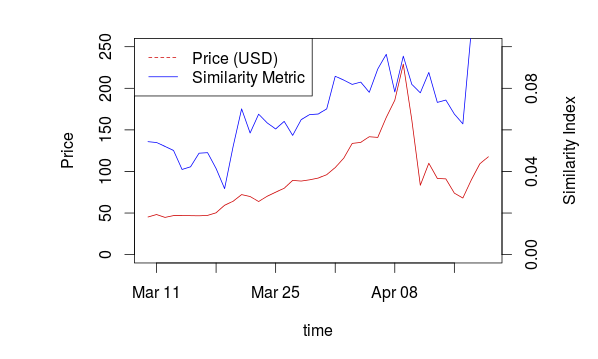
\includegraphics[width=100mm]{./figure/pnc.png}
\caption{Daily transactions price correlation with network structure. }
\label{fig:close_transactions}
\end{center}
\end{figure}

Visual inspection shows a good correspondence between price and similarity index, which is in line with the high high correlation coefficients (0.77) between two datasets.

\begin{figure}[ht]
\begin{center}
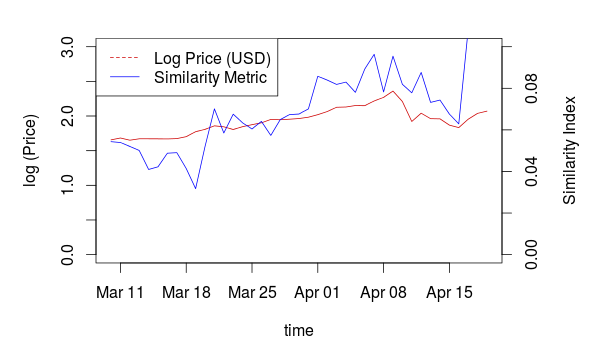
\includegraphics[width=100mm]{./figure/lpnc.png}
\caption{Daily transactions price (log) correlation with network structure.}
\label{fig:log_transactions}
\end{center}
\end{figure}

We plan to use other methods discussed in \citet{Vishwanathan2010} to check for expensive runtime $O(n^{6})$, tottering and halting \citep{Borgwardt2005} problem on above discussed method.

\section{Deep Graph Kernel}

Deep Graph Kernels \citep{Yanardag2015} is not so deep learning frame work to learn latent representations of sub-structures for graphs, which are not independent. The framework leverage on the dependency information between sub-structures by learning their latent representations. 

Graph Kernels are produced using R-convolution, where a graph is to recursively decomposed into into “atomic” sub-structures to define a kernels between them.  Mathematically, It can be expressed as:

%
\begin{equation}\label{eq:6.1}
K(G_{1}, G_{2}) = {\Bigg \langle \Phi(G_{1}), \Phi(G_{1}) \Bigg \rangle}_{\mathcal{H}}
\end{equation}
%
Where, $\Phi(G)$ is denote a vector which contains counts of atomic sub-structures. The representation in the equation \ref{eq:6.1} suffers from two basic problems. First, the sub-structure are not independent. Second, the dimension of the feature space often grows exponentially, as substructure grows, which leads to "diagonal dominance", that is, a given graph is similar to itself but not to any other graph in the dataset. But, we need a kernel matrix where all entries belonging to a class
are similar to each other, and dissimilar to everything else. To alleviate this problem, we define alternative graph kernel as:

%
\begin{equation}\label{eq:6.1}
K(G_{1}, G_{2}) = \Phi(G_{1})^{T} \mathcal{M} \Phi(G_{1})
\end{equation}
%
 
where $\mathcal{M}$ represents a $|\mathcal{N}|\times |\mathcal{N}|$ positive semi-definite matrix that encodes the relationship between sub-structures and $\mathcal{N}$ represents the vocabulary of sub-structures obtained from the training data. Now, the important task is design $\mathcal{M}$, which can be computed by learning latent representations of sub-structures or by edit-distance relationship between sub-structures. 

The language modeling and deep learning techniques was used to compute $\mathcal{M}$ with intuition that different
sub-structures compose graphs in a similar way that different words form sentences when used together. The list of decomposed sub-structures
for each graph is then treated as a sentence that is generated from a
vocabulary $\mathcal{V}$  where vocabulary $\mathcal{V}$ simply corresponds to the unique set of observed sub-structures in the training data. The linear co-occurrence relationship of sub-structure is created using modified random sampling scheme, taking account of neighborhoods. That is, whenever we randomly sample a graphlet $G$, we also sample its immediate neighbors. Then is corpus is generated according to particular graph kernels, for example, for shortest graph kernels, whenever shortestpath sub-structure is generated, all possible shortest-path
sub-structures are also collected that share the same source node, and treat them
as co-occurred.

Once corpus is generated, the model is build by using CBOW or Skip-gram algorithms and trained with Hierarchical softmax or negative sampling. If Let $s$ represent an arbitrary sub-structure from a vocabulary $\mathcal{V}$, and $\phi_{s}$ represent learned vector representation of $s$. Matrix $\mathcal{M}$ is calculated such that, each entry on the diagonal is $\mathcal{M}_{ii}$ computed as $\big \langle \phi_{i},\phi_{i} \big \rangle$ where $\phi_{i}$ corresponds
to learned d-dimensional hidden of sub-sequence $i$ and $\mathcal{M}_{ii}$
where $i = $j and $1 \leq i \leq |\mathcal{V}|$ (resp. $j$). After computing the $\mathcal{M}$ matrix, it is plugged in Equation \ref{eq:6.1} to get deep graph kernels.

The conducted experiments with diverse real life data, confirms that deep kernels improves the classification accuracy, robust to random noise and computationally efficient.

\section{Future Directions}
\label{sec:con}

In this report, we find strong correlation between structural property (walk) of bitcoin transaction graphs and BTC/USD exchange rate (price) by calculating similarity index using basic random walk graph kernels\citep{Gartner2003, Kashima2003}. 

As we find strong correlations ($\rho =7.7$) above, the same experiments is expected to performed taking other robust graph kernels in particular shortest path, free from tottering and halting problems. We intend to use "propagation kernels" \citep{Neumann2015}, which can be used to construct kernels for many graph types, including labeled, partially labeled, unlabeled, directed, and attributed graphs, considering we have weighted dircted labled attributed graph. This makes easy to extend our work taking account of attributes to do price forecast in future. 

Since, \citep{Yanardag2015} deep graph kernels outperforms popular graph kernels, we intent to use the same approach with modification in graph sampling and adding other graph kernels, especially propagation kernels \citep{Neumann2015}. We are also going to replicate the work in the paper with different datasets.

Though, we wanted to reproducing results from \citet{Kondor2014} studies, but that will depend on the time. But, we will  use \citet{Lee2015} graph similarity approach, based on random walk with restart (RWR) algorithm with intergraph compression to transform representation of graph for comparing it with graph kernels or its variant.


\newpage
\bibliographystyle{plainnat} 
\bibliography{./reference/ref}

\end{document}

